\chapter{综合实验}

本章首先对第\ref{chapter-Data}章中获取的地图数据正确性进行了分析验证,以确保上传给区块链的真实地图数据可信。接下来以基于树状区块链的出租车调度系统为载体进行综合实验。经过本文工作完善后的出租车调度系统能够根据路况动态地规划路径,表明了本文提出算法的可应用性;在实验过程中获取的数据证明了结合实时路况的改进A*算法具有良好的时间复杂度与空间复杂度,证明了把基于实时路况的改进A*算法引入出租车调度系统这一行为具有可行性。

在本章的实验中,区块链服务端和客户端均部署在虚拟机内,配置环境为:

1.虚拟机软件:7.0.6版本的VirtualBox

2.虚拟机的Linux操作系统:22.04版本的Ubuntu。

3.虚拟机基础配置:(1)内存大小为5220MB;(2)4核处理器;(3)磁盘空间为30.00G。

本章实验中所对应的数据文件存放的Github地址见附录D。

\section{地图数据的正确性验证}

本文在第\ref{chapter-Data}章中一共准备了五份地图,分别为out\_wx4e.json、out\_wx4eq.json、out\_wx4er.json、out\_wx4en.json、out\_wx4ep.json。

由Geohash编码的特征可知,一个Geohash编码父区域所对应的Geohash值一定是该区域的子区域编码值的前缀。本文导出的五份地图中,out\_wx4e.json是out\_wx4eq.json、out\_wx4er.json、out\_wx4en.json、out\_wx4ep.json这四份子地图的父区域,每份子地图中含有几千条路段,每个路段会包含不同的经纬度点位,这些经纬度点位经由Geohash编码后,也以子地图区域的编码值为前缀。因此,定义以下四个名词:

\begin{enumerate}
    \item 数据总量:指当前地图文件中,所有Geohash编码数据的个数。
    \item 有效数据:指统计点位的Geohash值前缀与当前地图父区域的Geohash值相同的数据。此时认为该点位属于此地图父区域,该点位是有效数据。
    \item 无效数据:指统计点位的Geohash值前缀与当前地图父区域的Geohash值不同。此时认为该点位不属于此地图父区域,该点位是无效数据。
    \item 可信度:指在一份地图文件中,有效数据在数据总量中的占比。
\end{enumerate}

对五份地图数据中包含的点位进行统计,得到图\ref{mapdataanalysis-pic}中的结果,对该结果的解释和分析如下。

\begin{figure}[ht]
  \centering
  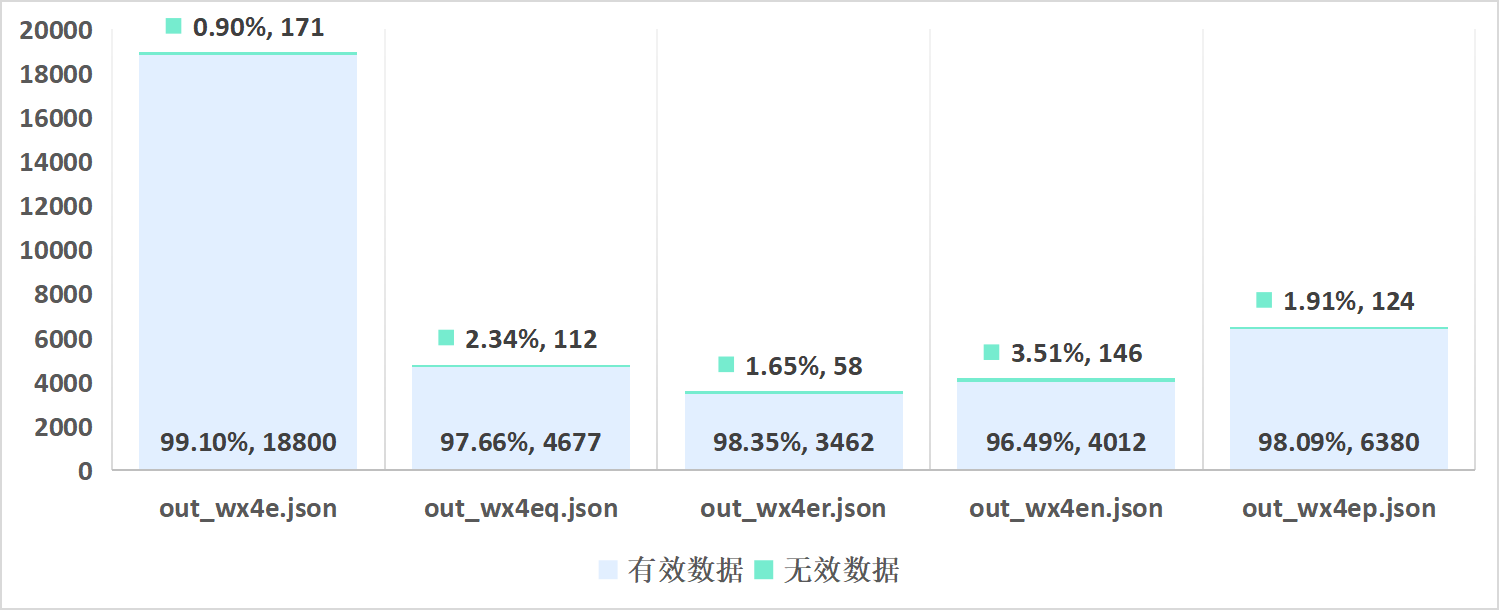
\includegraphics[width=0.9\textwidth]{undergraduate-thesis/images/mapDataAnalysis.png}
  \caption{第\ref{chapter-Data}章中有效地图数据占比图}
  \label{mapdataanalysis-pic} % label 用来在文中索引
\end{figure}

1.out\_wx4e.json地图:

此地图文件中:数据总量为18971;有效数据指以wx4eq、wx4er、wx4en、wx4ep为前缀的Geohash编码数据,其共有18800项,在数据总量中占比99.10\%;无效数据指以wx4g、wx4d、wx4ew、wx4em、wx4ej、wx4ex为前缀的Geohash编码数据,其共有171项,在数据总量中占比0.90\%。因此本地图文件可信度为99.10\%。

2.out\_wx4eq.json地图:

此地图文件中:数据总量为4789;有效数据指以wx4eq为前缀的Geohash编码数据,其共有4677项,在数据总量中占比97.66\%;无效数据指以wx4er、wx4em、wx4ew、wx4en为前缀的编码数据,其共有112项,在数据总量中占比2.34\%。因此本地图文件可信度为97.66\%。

3.out\_wx4er.json地图:

此地图文件中:数据总量为3520;有效数据指以wx4er为前缀的Geohash编码数据,其共有3462项,在数据总量中占比98.35\%;无效数据指以wx4eq、wx4ep、wx4ex、wx4g为前缀的编码数据,其共有58项,在数据总量中占比1.65\%。因此本地图文件可信度为98.35\%。

4.out\_wx4en.json地图:

此地图文件中:数据总量为4158;有效数据指以wx4en为前缀的Geohash编码数据,其共有4012项,在数据总量中占比96.49\%;无效数据指以wx4eq、wx4ep、wx4ej、wx4d为前缀的编码数据,其共有146项,在数据总量中占比3.51\%。因此本地图文件可信度为96.49\%。

5.out\_wx4ep.json地图:

此地图文件中:数据总量为6504;有效数据指以wx4ep为前缀的Geohash编码数据,其共有6380项,在数据总量中占比98.09\%;无效数据指以wx4er、wx4en、wx4g、wx4d为前缀的编码数据,其共有124项,在数据总量中占比1.91\%。因此本地图文件可信度为98.09\%。

\begin{figure}[ht]
  \centering
  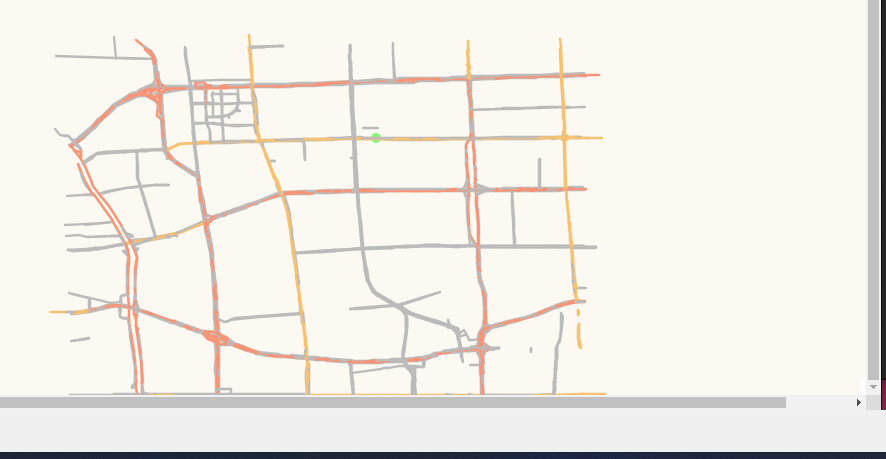
\includegraphics[width=0.8\textwidth]{undergraduate-thesis/images/2023-05-16 (7).png}
  \caption{out\_wx4e.json地图可视化效果}
  \label{wx4esuccess} % label 用来在文中索引
\end{figure}

由数据分析可知,五份地图文件的可信度分别依次为99.10\%、97.66\%、98.35\%、96.49\%、98.09\%。因此,认为第\ref{chapter-Data}章中给出的地图文件是正确可信的。

向系统中导入out\_wx4e.json数据后,其可视化效果如图\ref{wx4esuccess},证明本文中获取地图数据的过程是正确的;以out\_wx4eq.json地图数据为基础,在调度系统中完成一轮运行的成功图像如图\ref{wx4eqsuccess}所示,证明本文导出的地图数据能支持调度系统运行。

\begin{figure}[ht]
  \centering
  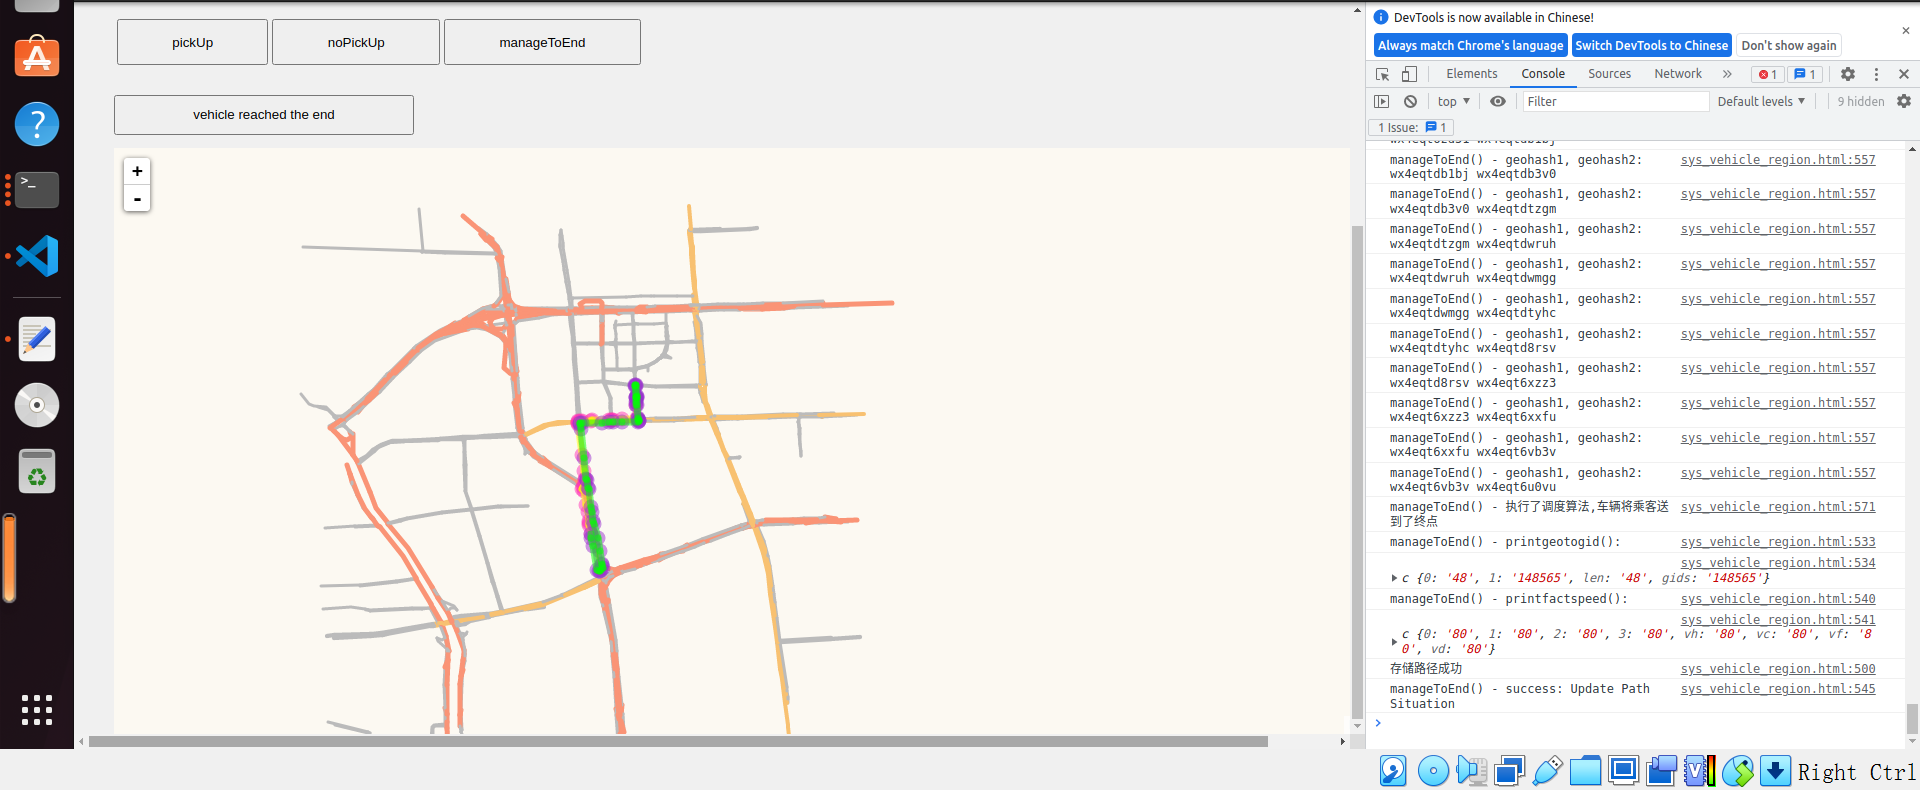
\includegraphics[width=0.9\textwidth]{undergraduate-thesis/images/2023-05-16 (12).png}
  \caption{out\_wx4eq.json上的运行效果}
  \label{wx4eqsuccess} % label 用来在文中索引
\end{figure}


\section{运行实验}
\label{runEx}

本节使用树状区块链的单子链,在方格地图上进行了基于改进A*算法的出租车调度系统的运行实验。

在本实验中,使用的车辆初始位置为:wx4erjmbekd(用绿色圆形标注);采取的乘客起点位置为:wx4erxjzekd(用蓝色圆形标注);采取的乘客终点位置为:wx4erjmbekd(用红色圆形标注)。在运行过程中,传统A*路径规划算法一共被调用2次,第1次是pickUp()过程,车辆从初始位置前往乘客起点,用黄色线条表示路径;第2次是manageToEnd()过程,车辆从乘客起点前往乘客终点,用绿色线条表示路径。

\subsection{使用传统A*算法的调度系统运行结果}

\begin{figure}[ht]
  \centering
  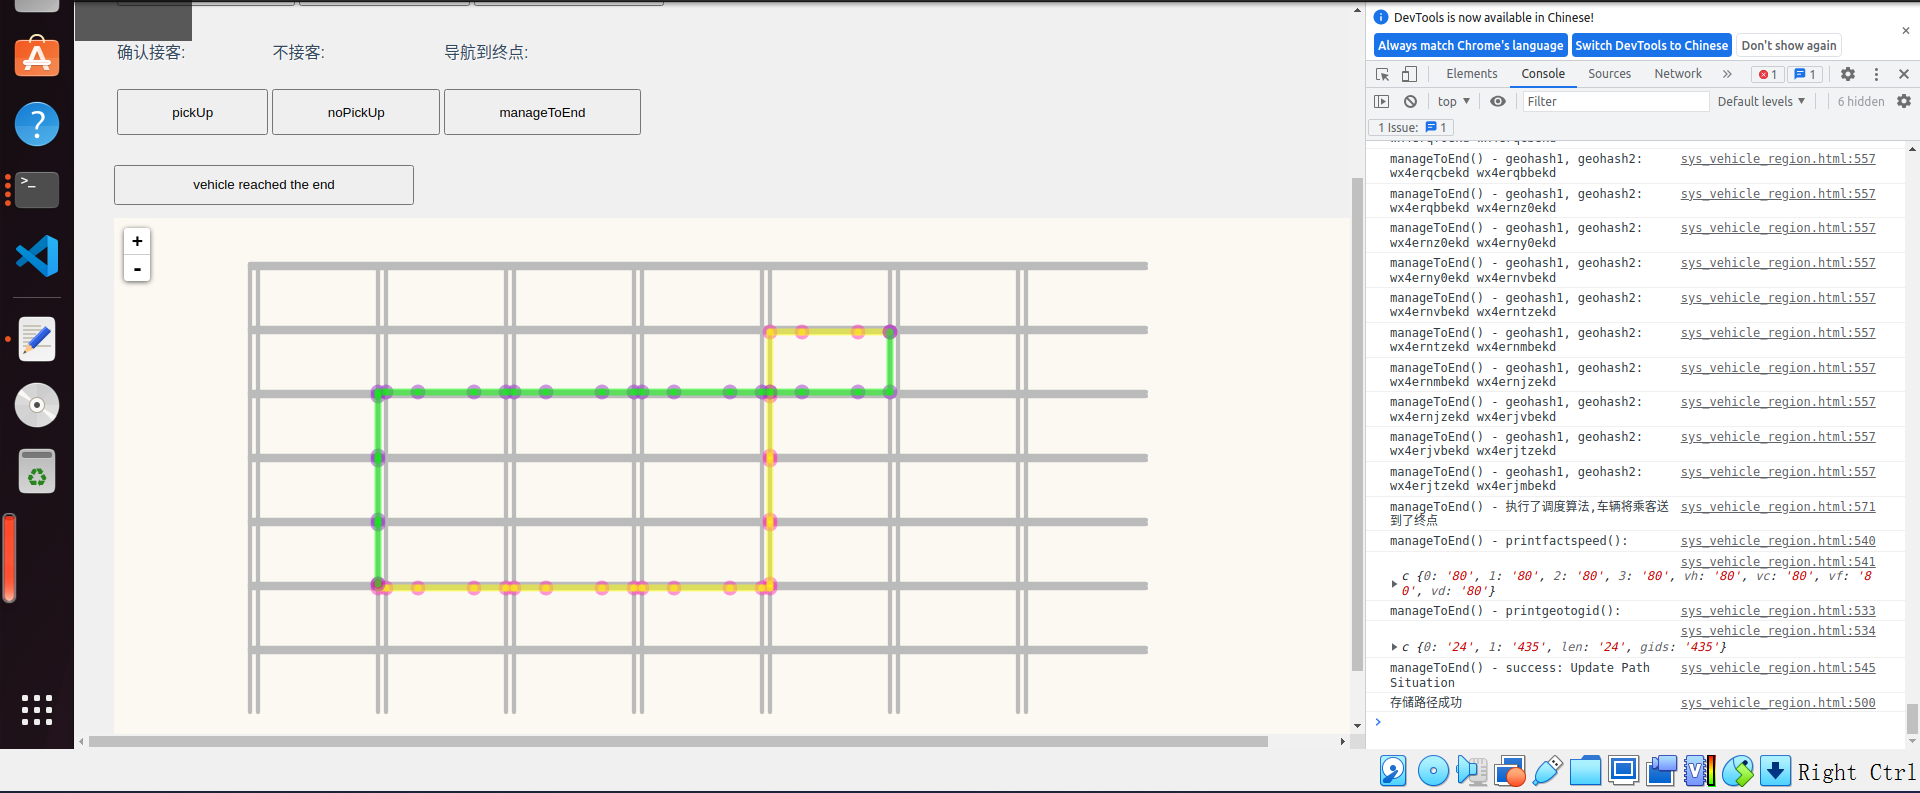
\includegraphics[width=0.9\textwidth]{undergraduate-thesis/images/2023-05-16 (1).png}
  \caption{使用传统A*算法的调度系统运行结果}
  \label{nine-old-Taxi} % label 用来在文中索引
\end{figure}

图\ref{nine-old-Taxi}中在pickUp()阶段和manageToEnd()阶段的总距离代价分别为3107和3069,这两个阶段规划出的结果如附录中的表\ref{exper1}所示。

使用传统A*算法的调度系统不考虑路况信息,只考虑道路距离,因此,无论运行多少次,只要区块链上部署的地图、车辆位置、乘客起点终点保持不变,则调度系统规划的黄色pickUp()路径和绿色manageToEnd()路径不会发生变化。

\subsection{使用改进A*算法的调度系统运行结果}

本文在智能合约中基于实时路况对A*算法完成了改进。在改进A*算法应用进出租车调度系统时,本文在智能合约与终端中进行以下假设:

1.路段的缺省速度为$V_{default}=80$km/h;

2.路段在第一次更新实时路况时保持通畅,即保持$V_{Current,1}=80$km/h。

3.在第n次更新实时路况时,如果有车辆在manageToEnd()阶段驶过某路段,将设定该路段的$V_{Current,n}=40$km/h,其中,$n\ge 2$。

4.在使用calPathCostToAdd()计算路段的实时路况代价时,设定公式\ref{cal-C(n)}中$\beta=15$,此举为了有效增加路段的实时路况代价,从而让运行结果有快速且明显的变化。

5.每轮运行一辆车、一位乘客,乘客发出一个订单,乘客完成支付、订单结束,则系统的本轮运行结束。

6.车辆位置、乘客的起点终点在不同轮次之间保持不变,此举的目的是能观察到不同轮次的实时路况对同一组位置的道路规划过程进行影响的变化效果。

基于以上六条假设,本系统进行了15轮运行,本文将对这15轮运行的结果从路况、道路成本代价两方面进行分析,并给出代表性的运行效果图。

\begin{figure}[ht]
  \centering
  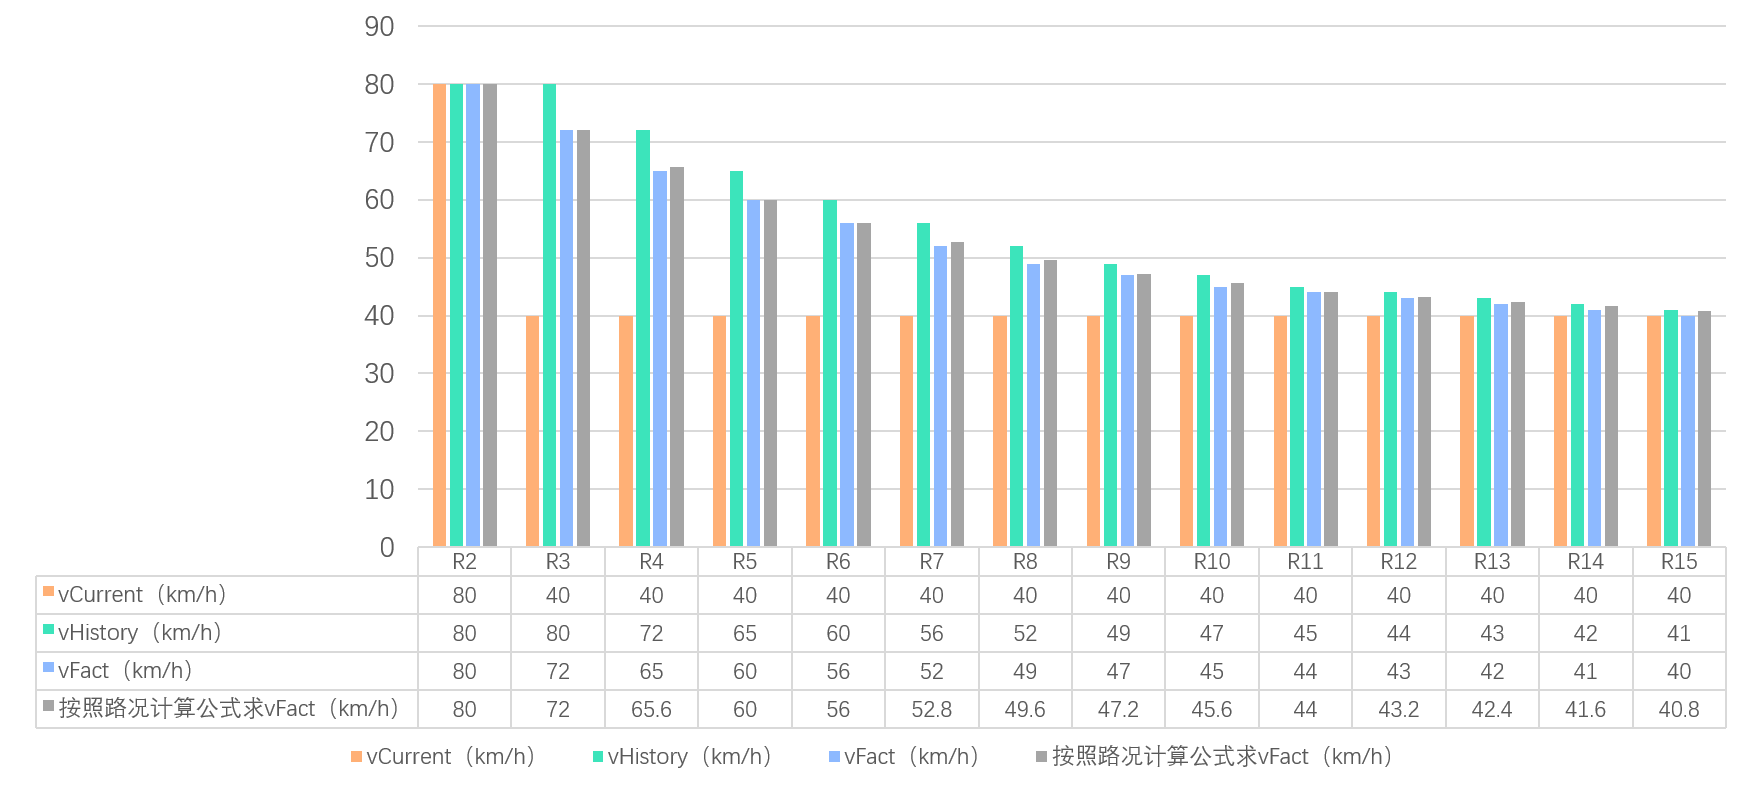
\includegraphics[width=1\textwidth]{undergraduate-thesis/images/PathSituationAnalysis.png}
  \caption{路况数据统计图}
  \label{nine-new-Taxi-path} % label 用来在文中索引
\end{figure}

图\ref{nine-new-Taxi-path}统计了第2轮次到第15轮次的道路速度数据,其中包括$V_{Current,n}$、$V_{History,n}$、$V_{Fact,n}$、$V_{default}$,由于$V_{default}$为道路的初始缺省速度,其一直保持不变,因此未在图\ref{nine-new-Taxi-path}中进行统计对比。

每次实时路况更新后,$V_{Current,n},(n\ge 2)$都为40,符合假设。

$V_{History,n}=V_{Fact,n-1}$,符合路况更新公式\ref{calpathSituation}。

根据公式\ref{calfact}:$V_{Fact,n}=V_{History,n}*0.8+V_{Current,n}*0.2$计算出的$V_{Fact,n}$如灰色数据所示,其与区块链上存储的数据$V_{Fact,n}$有较小差距。该差异出现的原因是:Solidity版本更新速度快,不同版本间的语法差异较大。本文使用的编译版本为0.5.17,该版本中的智能合约只能存储整数,不支持小数运算,因此在合约中实现公式\ref{calfact}时实际采用的计算公式为公式\ref{real-calfact},且计算出的$V_{Fact,n}$在区块链中只存储整数部分。
\begin{equation}
    V_{Fact,n}=(V_{History,n}*8+V_{Current,n}*2)/10
\label{real-calfact}
\end{equation}

数据证明,计算公式\ref{real-calfact}保留整数的效果较好,在无法存储小数的情况下能真实地逼近理想化的公式\ref{calfact}的计算结果,在区块链端进行数据存储。

\begin{figure}[!ht]
  \centering
  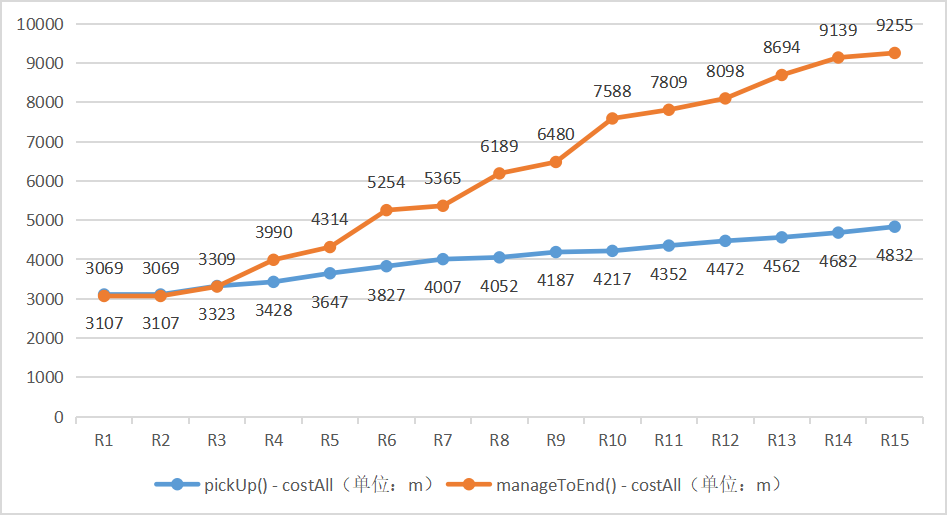
\includegraphics[width=1\textwidth]{undergraduate-thesis/images/CostAllAnalysis.png}
  \caption{改进A*算法在路径规划过程中的总距离成本数据统计图}
  \label{nine-new-Taxi-cost} % label 用来在文中索引
\end{figure}

本系统的调度过程分为两个阶段,第一个阶段是pickUp()过程,第二个阶段是manageToEnd()阶段。第一个阶段对车辆位置与乘客起点间进行路径规划,不调用updatePathSituation()更新实时路况,第二个阶段对乘客起点与乘客终点间进行路径规划,调用updatePathSituation()更新实时路况。costAll用于表示A*算法在路径规划过程中的总距离成本。在使用传统A*算法的调度系统的运行过程中,costAll和规划路径永远不变;在使用改进A*算法的调度系统的运行过程中,它的变化过程如图\ref{nine-new-Taxi-cost}所示。

在合约模拟道路速度的部分,只限定了路况拥堵状态,即车辆的运行导致路况从通畅变为拥堵,并未设计模拟道路由拥堵变成通畅的过程,因此costAll只会增加。pickUP()和manageToEnd()的costAll自第2轮开始都单调递增,这符合合约中模拟用例的预期效果。

pickUP()和manageToEnd()过程的costAll增长幅度不一致,前者增长速度缓慢且均衡,后者增长得越来越快。原因在于pickUp()过程未更新实时路况,其总距离成本costAll只会在manageToEnd()过程中走过的地方增加,增加的路段数量少,因此pickUp()的costAll增长慢且均匀。manageToEnd()每运行一次就会对此过程规划的每一段路段都增加拥堵效果,因此每运行一次,就会将该路段上所有位置的实时路况代价提高,提高的区域多,所以costAll增长比较快速。符合合约中模拟用例的预期效果。

\begin{figure}[!ht]
  \centering
  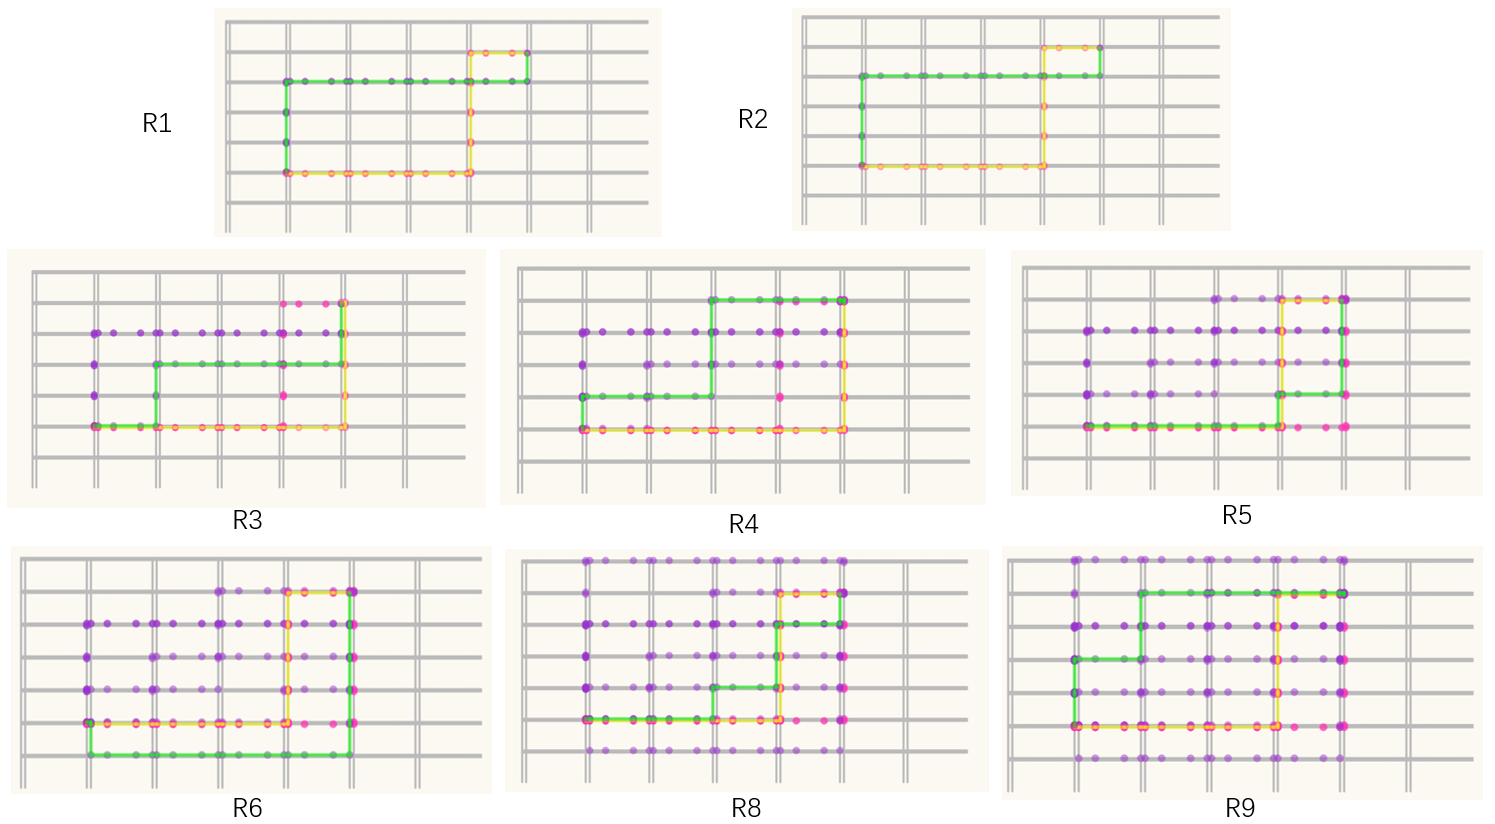
\includegraphics[width=1\textwidth]{undergraduate-thesis/images/2023-05-17.png}
  \caption{使用改进A*算法的调度系统运行结果示例}
  \label{nine-new-Taxi-pic1} % label 用来在文中索引
\end{figure}

图\ref{nine-new-Taxi-pic1}给出了本系统第1、2、3、4、5、6、8、9轮运行过程中的截图,该图中存在不同颜色的标识,各标识含义如下:黄色路径为pickUp()过程给出的路径规划结果;绿色路径为manageToEnd()过程给出的路径规划结果。黄色路径与绿色路径在路径规划结束后出现,在本轮订单完成后消失。粉色点线是pickUp()驶过的所有路径,紫色点线是manageToEnd()驶过的所有路径。当黄色路径出现时,粉色点线同时出现;当绿色路径出现时,紫色点线同时出现。车辆浏览器终端保持开启的时间段内,粉色点线和紫色点线不会消失;车辆浏览器终端重启,则粉色点线和紫色点线随之清零,并从零开始显示。设计不同颜色的路线,主要用于对比路径规划结果的区别。用粉色和紫色点线代表旧的路径规划路线结果,用黄色和绿色线段代表本轮的新路径规划路线结果,可视化表明第n轮规划出的新路线与第n-1轮规划出的旧路线基于实时路况发生变化。

在图\ref{nine-new-Taxi-pic1}中,由于$R1$、$R_2$轮次中道路路况均保持通畅,因此这两轮的calPathCostToAdd()计算结果都为0,则此两轮运行时,实时路况对道路规划的结果存在影响,但由于道路通畅,所以不改变道路规划结果。在$R_2$轮次结束之后,每轮运行都会使道路出现拥堵状况,因此实时路况会改变道路规划结果,新路径规划结果所对应的总距离成本代价值costAll在图\ref{nine-new-Taxi-cost}中得到统计,规划出的新路径在图\ref{nine-new-Taxi-pic1}中可视化表现。粉色、紫色路径在之前轮次被选出后,附加了道路拥堵状态,因此新轮次中如果继续按照粉色、紫色路径运行,道路成本将会升高,所以改进A*算法会规划出与其不同的黄色、绿色路径,作为道路成本最低的新路径,供车辆行驶。

%总结一下实验的结论,强调一下实验结果

在传统A*算法的控制下,本系统给出的路径规划结果只关注路径长度这一个因素,因此永远不变,其寻得路径如图\ref{nine-old-Taxi}所示,该路径规划结果中包含的Geohash编码如附录C中表\ref{exper1}所示;在改进A*算法的控制下,本系统给出的路径规划结果关注实时路况与路径长度这两个因素,由于实时路况在不断变化,因此路径规划结果也会不断变化,这符合现实生活中司机根据当前道路拥堵而选择其他较通畅道路的场景。

\section{性能实验}
% ----- 更新实验
本节在第\ref{runEx}节的基础上,使用了与运行实验相同的地图数据和车乘位置数据,并采取了相同的区块链服务端部署方式,但在终端部分使用JaveScript脚本通过web3接口直接与智能合约进行交互,以便于统计数据。本实验连续运行50轮出租车调度系统,获取到了50组运行数据。本节对这50组数据从不同角度进行了分析,综合评价了改进A*算法在应用进出租车调度系统后的性能,验证了本文改进的调度系统的可行性。

本实验关注以下两个性能指标:更新实时路况的时间损耗、改进A*算法的复杂度。

\subsection{更新实时路况的时间损耗}

本小节分析了在方格地图上运行使用改进A*算法的出租车调度系统,更新实时路况的时间损耗数据。该时间损耗发生在从终端的测试脚本里调用合约中更新实时路况的整个过程中,本文统计了系统每一轮运行过程中,调用合约里更新实时路况的全过程用时,并采用系统每一轮运行中的其他阶段用时作为对比数据。

\begin{figure}[ht]
  \centering
  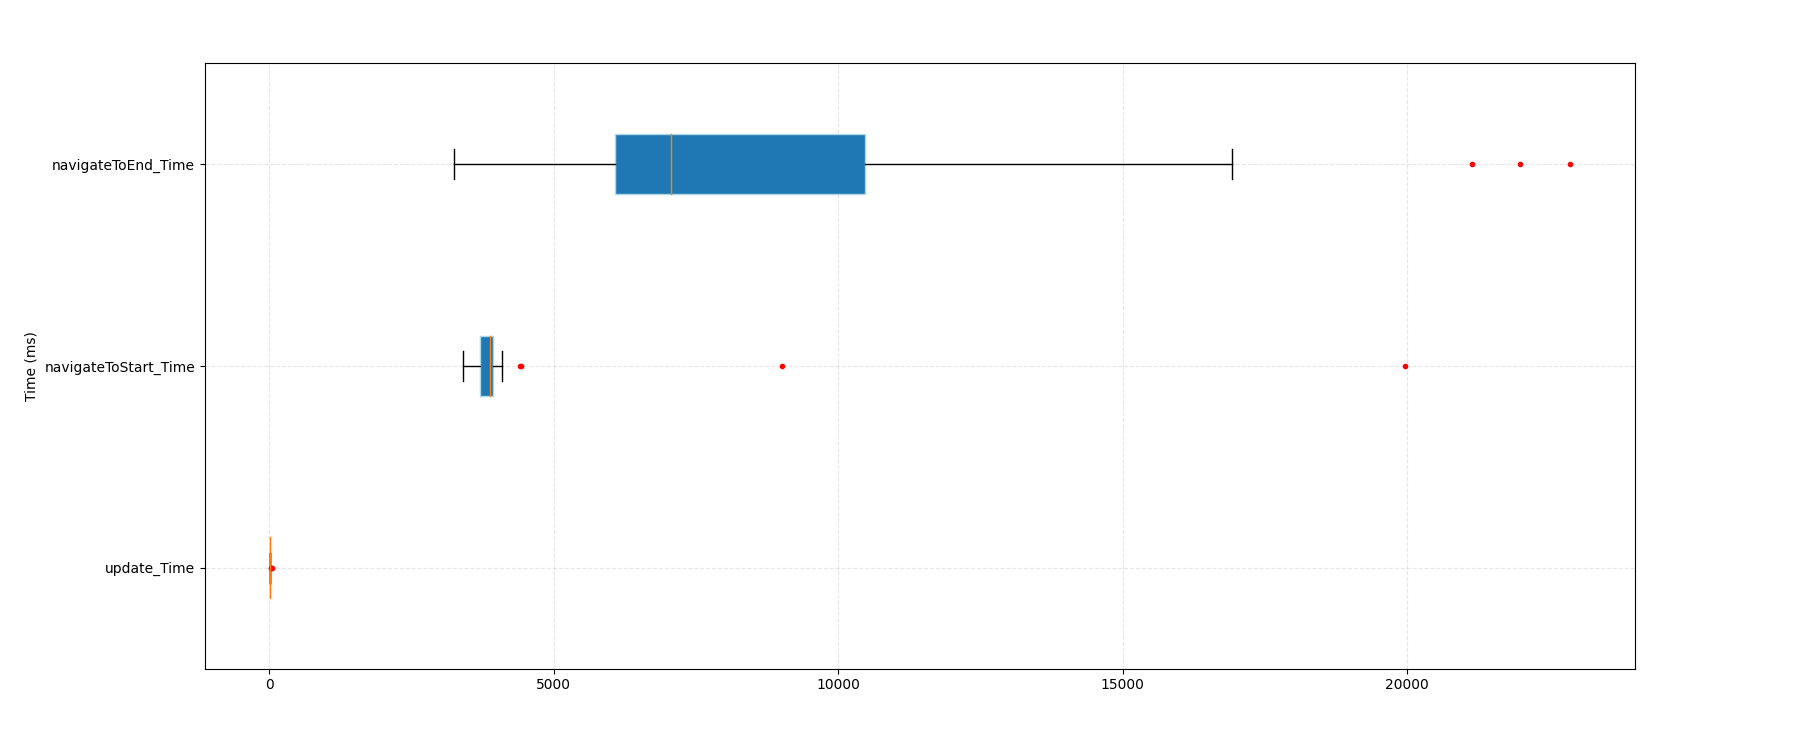
\includegraphics[width=1\textwidth]{undergraduate-thesis/images/2023-05-22 (2).png}
  \caption{系统运行不同阶段的时间损耗对比(单位:ms)}
  \label{nine-new-Taxi-time} % label 用来在文中索引
\end{figure}

图\ref{nine-new-Taxi-time}中展示了更新实时路况(update\_Time)、规划车辆前往乘客起点的路径(navigateToStart\_Time)、规划车辆从乘客上车到前往目的地的路径(navigateToEnd\_Time)这三个阶段的时间损耗数据,单位为ms。

update\_Time的中位数为10ms,平均值为10.82ms;navigateToStart\_Time的中位数为3882ms,平均值为4253.96ms;navigateToEnd\_Time的数据中位数为7225ms,平均值为8803.36ms。

可见,update\_Time的用时损耗占车辆前往乘客起点时间的0.25\%左右,占车辆接到乘客后前往乘客终点时间的0.13\%左右。在车辆通过智能合约规划路径时,需要借助合约中的A*算法进行路况调度,其借助区块链服务端的数据进行了大量运算,耗时较长;在车辆更新实时路况时,在区块链服务端中修改数据量较小,不需访问大量数据,因此耗时极短。

这说明,在基于树状区块链的出租车调度系统添加更新实时路况的环节后,该环节几乎不影响整个系统的运行时间,因此证明了本文所改进的实时路况计算部分具有极高的可行性。

\subsection{改进A*算法的复杂度}

\begin{figure}[ht]
  \centering
  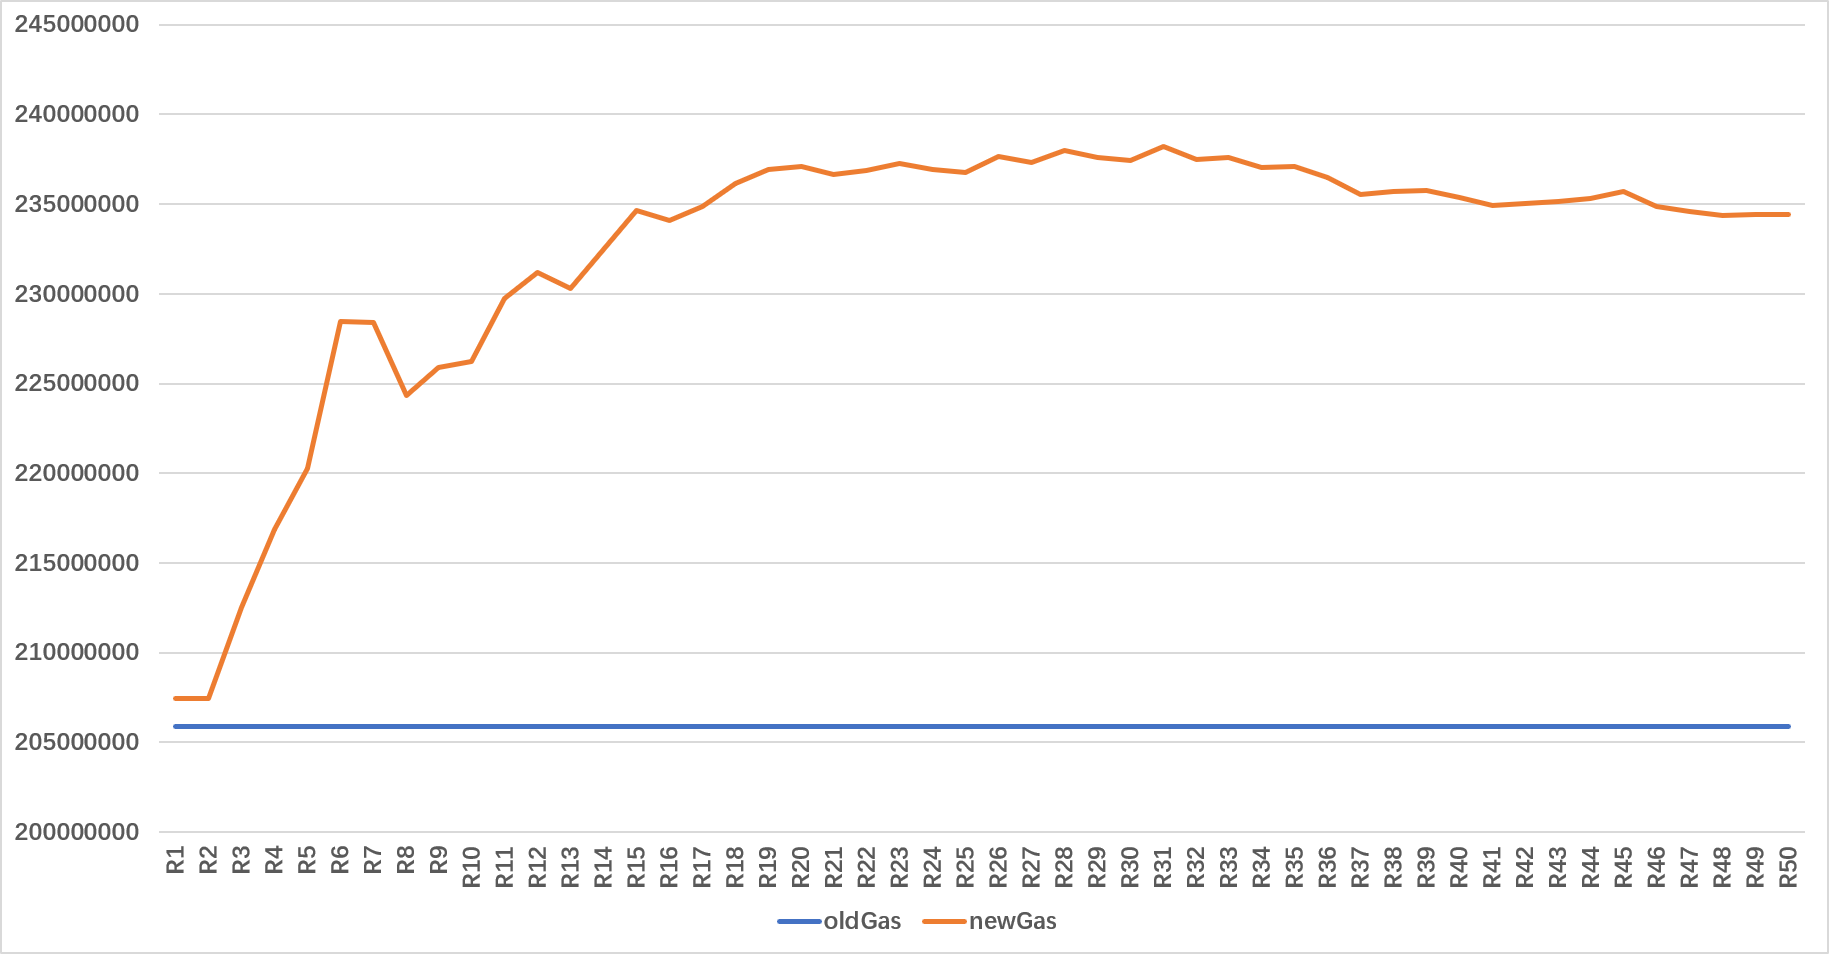
\includegraphics[width=0.8\textwidth]{undergraduate-thesis/images/gasData.png}
  \caption{改进前后A*算法的gas消耗}
  \label{nine-new-Taxi-gas} % label 用来在文中索引
\end{figure}

在区块链中,每笔智能合约的运行都需要支付一定量的gas,该gas的多少取决于智能合约的复杂度。因此,本节统计了智能合约运行过程中gas值的损耗量,用该数据量化代表A*算法的复杂度,对比传统A*算法消耗gas量与改进A*算法消耗gas量,作为改进A*算法的复杂度参考。

图\ref{nine-new-Taxi-gas}展示了传统A*算法和改进A*算法在被调用时消耗的gas量,oldGas线对应传统A*算法的gas损耗,newGas线对应改进A*算法的gas损耗。

该图像反映3个可关注信息:1. oldGas线为水平直线;2. newGas线整体高于oldGas线;3. newGas线整体的走势为增长趋势,且前半段爬升较快,后半段趋于稳定,以第$Round_{16}$轮次为界。对这些信息的分析如下:

\begin{enumerate}
    \item 图中oldGas线对应的数据为定值,在图像中表现为一条水平直线,这是因为:在使用传统A*算法的出租车调度系统运行过程中,由于传统A*算法只根据道路长度规划路径,因此每次的计算量是固定的,则算法复杂度也是固定的,量化为gas值损耗后,其gas损耗也为定值205910896,这符合图像中oldGas线的趋势。
    \item 图中newGas线整体高于oldGas线,这是因为:在使用改进A*算法的出租车调度系统运行过程中,由于改进A*算法将实时路况纳入计算因素,每轮规划完路径后会同步更新路况,因此区块链中存储的路况数据将不断增长,因此newGas线整体高于oldGas线,这证明改进A*算法的整体计算量和复杂度要高于传统A*算法。
    \item newGas线整体走势为增长趋势,且前半段变化剧烈,后半段趋于稳定,以第$Round_{16}$轮次为界,这是因为:(1)随着实时路况的计算,区块链中存储的数据不断增长,在调用改进A*算法时,对应的计算量也随之呈现整体上的增长趋势;(2)但根据计算,在第$Round_{15}$轮次路况更新结束之后,计算的$V_{fact,15}$已收敛到$V_{current,i}(i>=2)$对应的40km/h,因此区块链段更新的数据量较第$Round_{16}$轮以前有所减少,在调用改进A*算法时的计算量逐渐趋于稳定。该newGas线对应的数据符合智能合约中的行为及实时路况模拟行为,因此证明改进A*算法在本系统中运行合理且正常。
\end{enumerate}

在50轮的运行中,newGas的平均值为232461650.76,相比于oldGas来说提高了12.89\%。该数据说明在当前实时路况模拟的状态下,改进A*算法的复杂度较传统A*算法来说提高了12.89\%左右,该复杂度的提升尚可接受。相比于传统A*算法而言,改进A*算法提升了较低的复杂度,但能实现路径的动态规划效果,因此使用改进的A*算法对本文中提及的出租车调度系统进行完善是具有可行性的。

\section{本章小结}

首先,本章对本文处理的真实地图数据的正确性以统计的方式进行了分析与验证,以确保上传给区块链的地图数据符合北京道路特征,并且在系统中对真实地图数据进行可视化显示,保证了地图数据的可用性与正确性。

接着,本章使用方格地图数据,对使用传统A*算法的调度系统与使用改进A*算法的调度系统分别进行了运行实验与性能实验:1. 运行实验证明了改进A*算法在出租车调度系统中的可运行性。2. 性能实验的结果表明,结合实时路况的改进A*算法拥有良好的时间和空间复杂度,尽管改进A*算法相比于传统A*算法会提升一定的运算代价,但舍弃该代价能将路径规划由静态转为动态,更符合真实的出租车调度过程,为了模拟真实的调度场景,该代价是可接受的。本章的运行实验与测试实验证明了本文改善的出租车调度系统的可行性。
